\hbadness=10000
\vbadness=10000

\def\epsilon{\varepsilon}
\def\phi{\varphi}
\def\bool{\{0,1\}}
\def\poly{{\sf poly}}
\def\cross{\times}

\newcommand{\xor}{\oplus}
\newcommand{\Xor}{\bigoplus}
\newcommand{\ceil}[1]{\left\lceil {#1} \right\rceil}
\newcommand{\floor}[1]{\left\lfloor #1 \right\rfloor}
\newcommand{\ignore}[1]{}
\newcommand{\integers}{{\mathbb Z}}
\newcommand{\naturals}{{\mathbb N}}
\newcommand{\bydef}{\stackrel{\rm def}{=}}
\newcommand{\isequal}{\stackrel{\rm ?}{=}}
\newcommand{\compeq}{\stackrel{\rm c}{\equiv}}

\newcommand{\qed}{\hspace*{\fill}\rule{7pt}{7pt}}
\newenvironment{proof_sketch}{\noindent{\bf Sketch of Proof} (Informal)\hspace*{1em}}{\qed\medskip}
\newenvironment{proof}{\noindent{\bf Proof}\hspace*{1em}}{\qed\medskip}
\newenvironment{proofof}[1]{\noindent{\bf Proof} of #1:\hspace*{1em}}{\qed\medskip}
\newenvironment{claim}{\noindent{\bf Claim}\hspace*{1em}\begin{em}}{\end{em}\medskip}
\newcounter{defcounter}
\setcounter{defcounter}{1}
\newenvironment{definition}{\medskip\noindent{\bf Definition \thedefcounter}}{\hspace*{\fill}$\diamondsuit$\stepcounter{defcounter}\medskip}
\newtheorem{theorem}{Theorem}
\newtheorem{corollary}[theorem]{Corollary}
\newtheorem{lemma}[theorem]{Lemma}
\newtheorem{claim_}[theorem]{Claim}
\newtheorem{fact}[theorem]{Fact}
\newtheorem{conjecture}[theorem]{Conjecture}
\newenvironment{assumption}{\noindent{\bf Assumption}\hspace*{1em}\begin{em}}{\end{em}\medskip}
\newenvironment{remark}{\noindent{\bf Remark}\hspace*{1em}}{\bigskip}
\documentclass[11pt, english]{article}
\usepackage{graphicx, textcomp, seqsplit, cite, tikz, latexsym, float, changepage}
\usepackage{caption, enumitem, amsmath,amssymb,amsthm,listings,hyperref, titlesec}
\usepackage{lettrine, pdfpages, lscape, multicol, blindtext, amsfonts, xcolor}
\usepackage[square,numbers]{natbib}
\usepackage[bottom]{footmisc}
\usepackage[most]{tcolorbox}
\setlength\columnsep{.5in}
\pagenumbering{arabic}
\graphicspath{{imgs/}}
\usepackage[a4paper,
    bindingoffset=0in,
    left=0.75in,
    right=0.75in,
    top=1in,
    bottom=1.25in,
    footskip=.25in
]{geometry}

\begin{document}
\captionsetup[figure]{name=Fig.}
\pagecolor{yellow}
\thispagestyle{empty}

\vspace*{.2in}
\begin{figure}
    \centering
    \tcbox[boxrule=.5pt,boxsep=0pt,colback=white]{\includegraphics[width=240pt]{logo.png}}
\end{figure}

\vspace*{-.23in}

\begin{center}
    \parbox{4.5in}{
        \noindent{\small{\textit{
                Capital markets are supposed to facilitate the efficient formation of capital to support the expansion and growth of business and the creation of employment and prosperity for all of society.
                \\\textcolor{yellow}{.}
                \\But these days the exchanges are all for-profit businesses, and they all seem to be beholden to their best customers... who have the least to do with the purpose for which markets actually exist in the first place.
            }\\\rightline{--- Erik Townsend}}}
    }
\end{center}
\vspace*{.23in}



\begin{abstract}
  
  \noindent What if you didn't have to wait days for trades to clear, pay exorbitant hidden fees to your broker, or worry about holding counterfeit stock?\cite{Infrastructure_2021}\cite{Rebates_2015}\cite{Counterfeiting_2023}. Capital markets work, but they're incredibly inefficient. A few powerful institutions: 
  \begin{itemize}
      \item control stock lending and margin, generating fake shares en mass;\footnote{How can stocks reach their full market value with mass sales of non-existent shares? See Page \ref{the_problem}.}
      
      \item systematically disenfranchise global investors from buying stocks; \cite{Senate_1974,Funch_et_2003} and
      
      \item through manipulative systems, ultimately cost investors over \$3.75T/year.\footnote{We estimate these hidden fees cost the average stock investor 0.5\%/year (\$600k after \$1k/month/40 years in indexes).}
  \end{itemize}
  \vspace{.125in}
  
  Transfer agents can uproot industry behemoths by undermining their grasp on capital markets. In particular, all brokers are commingled as but a single investor on the books of public companies. Public firms hire a ``transfer agent'' to maintain these investor records.\\
  
  The stock transfer agent industry has consolidated to four major providers over the past few decades. Service amongst them has dwindled while prices skyrocket. Issuers are not satisfied.\\
  
  Old transfer agents force book-entry stockholders to print complex paperwork, travel to an approved bank, present identification documents, wait for a tedious banker review, snail mail everything, and hope for an unhurried account statement or check back.\footnote{This uses a ``medallion signature guarantee stamp.'' Most impoverished investors abroad can't access authorizing banks for this special certification, and online alternatives cost months of savings. Finance should be open to everyone. Investing should be simple no matter where you were born.}\\
  
  We think significantly more investors would use transfer agents if their trading experience was digital, streamlined, and came with easy bank connections. This is possible since private stock sales on your own behalf aren't regulated as stringently as traditional capital markets.\\
  
  Transfer agents haven't offered a trading interface because old market technology required centralized coordination. Securities laws disallow transfer agents from this. But decentralized ledgers and particularly the Stellar Decentralized Exchange (``\href{https://developers.stellar.org/docs/learn/encyclopedia/sdex/liquidity-on-stellar-sdex-liquidity-pools}{SDEX}'') let book-entry investors match trades from anywhere with zero middlemen.
\end{abstract}

\vspace*{.44in}

\begin{center}

\small{Provided in good faith for informational purposes only.}

\end{center}

\pagebreak
\pagestyle{plain}
\setcitestyle{numbers}
\setcounter{page}{1}



\section{Banks \& Brokers Decided Long Ago to put Profits Above Accuracy}\label{the_problem}
\large{
    \begin{itemize}
        \item Dole Foods went private for \$1.2B in 2013. The company only had 37M shares outstanding, but brokerage investors held 49M shares---12M extra. A third of the company’s supposed investors didn't get paid in a later class action. \cite{Kentouris_2017,Laster_2017}
        
        \item Just two investors bought $125\%$ of a real estate company's shares in 2005. \cite{Faulk_2005,Avery_2005}

        \item Investors voted $135\%$ of shares in a top US defense contractor's meeting. \cite{Racanelli_2018,Behrendt_et_2006}
        
        \item Investors acquired $120\%$ of Overstock.com shares in 2006. \cite{Economic_2006,Rodriguez_2006}

        \item Investors bought $105\%$ of GameStop shares in 2022. \cite{FTD_2022}
        
        \item A leading Wall Street nonprofit trade association found more shares voted than issued in $75\%$ of 2019 annual meetings. \cite{May_2019}
    \end{itemize}
}

\begin{multicols}{2}

When we assign all our trust to a few central bookkeepers, we grant them the power to decree data transparency, investor accessibility, and arbitrary economic rents.

\begin{figure}[H]
    \raggedleft 
    \tcbox[boxrule=0.5pt,boxsep=0pt,colback=white]{
      \includegraphics[width=\linewidth]{centralized.png}
    }
    \caption{Centralized Bookkeeping}
    \label{fig:centralized}
\end{figure}

Today, centralized transfer agents slow us down with mountains of paperwork. The nature of their centralized systems require high fixed compatibility costs and human interaction, which often means snail mail and phone calls. But, with a slight change, we think transfer agents are the future of capital markets. We're redesigning capital markets \hbox{\textit{without}} centralized middlemen to eliminate:
\begin{itemize}
    \item 3.75T/yr in hidden fees to investors,
    
    \item profiteering from artificial shares, and
    
    \item unequal access to investments abroad.
\end{itemize}



\section{This Yellowpaper}

We believe registered ownership (as in not held by rent-seeking brokers) will remedy:
\begin{itemize}
    \item the true costs of slow, opaque markets with hefty hidden spreads,
    \item unequal access to capital markets and commission-free investments, and
    \item drastically unequal returns on capital due to centralized asset managers.
\end{itemize}

\noindent This Yellowpaper details how to use: \begin{enumerate}
    \item digital assets \textit{as} a transfer agent's authoritative master securityholder file,
    
    \item cryptographic signatures in place of medallion signature guarantees, and
    
    \item digital text memos for censorship-free, trackable distributed proxy voting.
\end{enumerate}



\section{Digital Transfer Agent}

Old transfer agents use paperwork and centralized databases for stock ledgers, which means manual data manipulation for every transfer. But people aren't very reliable when it comes to extremely repetitive math or nuanced numerical systems.

Unfortunately, the industry is rife with agents making simple arithmetic errors despite one prevalent software suite provider. Moreover, slow response times from overworked agent representatives can frustrate issuers and investors alike.

Regulation gives agents three days to respond to ``routine'' transfers, meaning you already spent three days getting a medallion stamp. From the moment all your paperwork lands in their mailbox, an agent can sit on their hands for days until they get around to updating their ledger. It's even worse if you try to transfer ``non-routine'' restricted shares. 

\begin{figure}[H]
    \centering
    \tcbox[boxrule=0.5pt,boxsep=0pt,colback=white]{
      \includegraphics[width=180pt]{medallion.jpg}
    }
    \caption{A Medallion Stamp}
    \label{fig:decentralized}
\end{figure}


\subsection{Automation}

New cryptographic technology lets us use proven mathematics instead of paperwork and trusted central processors. Namely, distributed public ledgers enable global investing by giving everyone the same \textit{digital} trading rules.\footnote{Using "trade" for when an investor transfers shares in exchange for a simultaneous transfer of dollars.}

These new systems can drastically boost investor protection, voting transparency, and market confidence by eliminating hidden back-office errors and processing time. In particular, Stellar ledgers close about every five seconds. Marginally slowing down trading into SDEX batches curtails riskless arbitrage opportunities, enhances investor liquidity, and curbs market volatility. \cite{Veryzhenko_2017,Budish_2015,Chakrabarty_2015}

\subsubsection{General overview}

Distributed ledgers let us keep track of investor balances using time-tested algorithms that execute in seconds, 24/7/365.\footnote{In particular, we'll discuss our implementation using the Stellar network, which is about a decade old.}

Instead of manipulating Excel spreadsheets, digital assets use programmatic ``atomic execution.'' That means trades take full and immediate effect, or they fail. No waiting for mail. No hard-copy documents. No mystery counterparty delivering shares a week later. Just digital signatures.\footnote{Namely, users sign transactions with elliptic-curve cryptography which effect when distributed to peers.}

\subsubsection{Trust in math, not middlemen}

\begin{figure}[H]
    \centering
    \tcbox[boxrule=0.5pt,boxsep=0pt,colback=white]{
      \includegraphics[width=\linewidth]{decentralized.png}
    }
    \caption{Distributed Bookkeeping}
    \label{fig:decentralized}
\end{figure}

To join the network, investors just privately associate their identity with a cryptographic public key. In practice, investors complete standard identity verification onboarding and generate a Stellar keypair.\footnote{Since investors never share their private keys, only they can digitally sign transfers through a wallet.}

Once we confirm investor identities, we map them to the given public keys. These public addresses identify investors both internally for compliance and on the Stellar distributed ledger (but without the PII).


\subsection{Ledger balances \textit{as} capital books}

We can send investors initial shares from an old transfer agent or legacy broker, entirely on Stellar. Once stock assets land in an investor account, they're free to privately trade with other verified accounts.

That means we no longer reference the Excel spreadsheet from an old agent for reporting, voting, or dividends. Rather, we can now query balances, trade data, and historic votes via the perpetual, immutable decentralized network in real time.

From the investor's point of view, everything looks like a normal cash account with account balances, positional PNL, and instant settlement.\footnote{Gain or loss derived from SDEX fill prices or legacy cost basis communicated in distribution memo.}\footnote{Investors exit trades by referencing a specific basis tax lot in the memo of a closing private trade.} But behind the scenes, investors are protected against hidden share lending, trade internalization, and predatory order routing.

Most importantly, all this ownership data stays on the distributed ledger, existing as the public company's master securityholder file. That means issuers never have to coordinate with middlemen to query investor trends, statistics, or vote responses.

Public records let everyone track their assets with confidence, attest to holdings seamlessly, and gain trading visability. They also keep basic financial information in the hands of all users---not a select few governments, custodians, or insiders.

This fundamental software freedom enables the next generation of computerized, decentralized, and permissionless innovation. It gives masses of people the necessary tools to accumulate real savings and retirements.

\subsubsection{Impact}

Since anyone can instantaneously create a blockchain wallet, cryptographic signatures satisfy the SEC's nondiscriminatory transfer requirements. We'd even venture to say that pressing a few buttons on a phone is significantly more equitable than waiting half a day at the bank with two IDs, especially abroad.

\begin{figure}[H]
    \centering
    \includegraphics[width=120pt]{paperwork.jpg}
    \caption{Book-Entry Trade Bank Paperwork}
\end{figure}

Thus, investors not only get their assets instantaneously, but companies also open up their shares to billions traditionally disenfranchised from direct equity investing. That's a big deal for growth-seeking investors abroad waiting to compliantly stash their cash in quality stocks without mountains of paperwork and fees.


\subsection{Proxy voting through memos}

No transfer agent has yet tallied investor votes transparently. Rather, quite the opposite is commonplace. Intermediaries count proxy cards behind closed doors, allocate broker votes arbitrarily, and discard unsatisfactory votes without notice. \cite{Clayton_et_2018,Higgins_2015}

We propose an alternative to mailing proxy cards with secret ``control number'' codes for a black-box voting machine.

\subsubsection{General process}

Once voting opens up, we send investors standard proxy notices. But investors use our wallet app to vote instead of dialing a call center or mailing back a postcard.

In the background, we set up a voting address like ``demo*proxyvote.io.'' Then, in the app, investors select the company they want to vote for once reading proxy materials. They go through an interface with the voting items, selecting `for,' `against,' `abstain,' or `withhold' for each item, which gets mapped to a memo. If an investor voted for the first four director elections and against the next two propositions, their memo would be ``YYYYNN.'' Then, they just send 0.0000001 XLM to the voting address with this memo, receiving instantaneous confirmation.

At the meeting, you can simply reconcile vote results from public voting addresses with record-date shareholder balances. Anyone can tally up public transaction memos to verify final counts, and all votes have the same cryptographic security as transfers.



\section{Conclusion}

This Yellowpaper presented three major innovations we use to implement controllable electronic stock records on the Stellar distributed ledger. If you're a public company, we can take care of the whole process for you in just a few steps while handling ongoing investor support and SEC compliance. If you're an investor, we hope to serve your account well.


\subsection{We shouldn't exclude 7 billion people from investing}

Investors should trade directly through a registered transfer agent rather than the outdated brokerage industry. 

Brokers are innately very expensive. Put briefly, if you want to operate a broker, you have to pay for trading and holding broker-dealer registrations, internalization infrastructure, market depository fees, trading data fees, order-routing commitment contracts, clearing agency membership, daily settlement deposit expenses, trade matching documentation, internal controls and audits for fairness, and tons of other costs associated with trusted central order matching.

Subsequently, it makes sense that most brokers don't want to serve low-value investors abroad. It's just too costly. But when you transact directly on the books of a public company, you avoid all these operational costs (plus the hidden trading fees ultimately passed on to investors). By replacing an outdated reliance on medallion stamps with modern cryptography, we open investing to anyone, anywhere, anytime.

\end{multicols}

\begin{figure}[H]
    \centering
    \includegraphics[width=420pt]{msg-map.jpg}
    \caption{Medallion Signature Guarantee Participants \cite{MSG_2022}}
\end{figure}

\pagebreak
\begin{multicols}{2}

\footnotesize{
    \bibliography{bibliography}
    \bibliographystyle{abbrv}
}

\end{multicols}

\appendix



\section{How transfer agents undermine the big banks, brokers, and HFTs}\label{appendix-intro}

\begin{figure}[H]
    \centering
    \tcbox[boxrule=0.5pt,boxsep=-3pt,colback=white]{
      \includegraphics[width=380pt]{simplified.png}
    }
    \caption{Simplified View of Appendix \ref{appendix-brokers}}
\end{figure}
\pagebreak



\section{Where transfer agents fit in trade clearing and settlement}\label{appendix-brokers}


\subsection*{Acronyms}

\begin{itemize}
  \item \textbf{National Best Bid and Offer (NBBO):} The highest bid and lowest ask limit order unfilled for a stock according to merged data from national securities exchanges.
  
  \item \textbf{Payment for Order Flow (PFOF):} Payment from a central third-party market maker to a broker-dealer in exchange for unfulfilled trades. Once order flow is sold, the buying firm must fulfill the trade at \textit{any} price within the NBBO range for the last one second.\footnote{Top market makers trade in under 120 nanoseconds, enabling riskless arbitrage against your orders.}\footnote{Kickbacks from market makers are disclosed in brokers' quarterly 606 disclosures.}
\end{itemize}

\noindent\begin{tikzpicture}{.9\textwidth}
    \node (A) at (-15,1) {\textbf{You}};
    \node (B)[draw, align=left] at (-15,-1.5) {Your Central Broker-Dealer\\or Equivalent Institution};
    \node[draw, align=left] (C) at (-8,-5) {(Internalization) Can the broker-dealer fill this order at \\the NBBO or better (order improvement) from:\\(i) another client from our firm looking to sell the same\\ security simultaneously at market rates or better,\\(ii) a short-term inventory of held extra assets that we\\set up to fulfill orders like this with, or\\(iii) a predetermined specialty asset such as a secondary\\bond for which purchase has already been arranged};
    \node[draw, align=left] (D1) at (-8,-1.5) {Internalize the trade \& \\keep the spread};
    \node[draw, align=left] (G) at (-14.5,-11) {Central Exchange Order Book \& \\National Best Bid \& Offer or \\Equivalent for Less-Liquid Assets};
    \node (H) at (-12,-16) {To Next Diagram};
    \node (H) at (-4,-13.8) {Centralized Market Makers};
    \node (H) at (-7.8,-.5) {Centralized Brokers};
    \node[draw, align=left] (I) at (-5,-9) {Can we fill this through a third-party off-exchange \\market maker and get  filled at the NBBO or better?};
    \node[draw, align=left] (J) at (-4,-12.8) {Fill the trade off central\\exchanges \& keep PFOF};
    \node[draw, align=left] (K) at (-12,-15) {Send the trade to central exchanges\\to get filled in the national order book};
    \node (C1) at (-8,-7) {};
    \node (G1) at (-13,-10.25) {};
    \node (G2) at (-14,-10.25) {};
    \draw[thick,->] (A) -- (B) node[midway,sloped,right,rotate=90] {Send an order};
    \draw[thick,->] (B) -- (C) node[midway,sloped,above,rotate=0] {};
    \draw[thick,->] (C) -- (D1) node[midway,sloped,right,rotate=270] {Yes};
    \draw[thick,->] (K) -- (G) node[midway,sloped,above,rotate=0] {SIP Quotes};
    \draw[thick,->] (B) -- (G) node[midway,sloped,above,rotate=0] {Quote Request$_1$};
    \draw[thick,->] (G2) -- (C) node[midway,sloped,above,rotate=0] {Quote$_1$};
    \draw[thick,->] (C1) -- (G1) node[midway,sloped,above,rotate=0] {No — Request Quote$_2$};
    \draw[thick,->] (G) -- (I) node[midway,sloped,below,rotate=0] {Quote$_2$};
    \draw[thick,->] (I) -- (J) node[midway,sloped,right,rotate=75] {Yes};
    \draw[thick,->] (I) -- (K) node[midway,sloped,below,rotate=0] {No};
\end{tikzpicture}

\pagebreak
\thispagestyle{empty}

\begin{adjustwidth*}{-101}{}
    \begin{tikzpicture}
        % Participant nodes
        \node[draw] (centralExchange) at (-10,8.1) {Home Exchanges};
        \node[draw] (exchangeBook) at (-10,7.435) {Exchange Order Book};
            \draw (-12,7.1) -- (-8, 7.1) -- (-8, 5.5) -- (-12, 5.5) -- (-12,7.1);
            \draw (-10,7.1) -- (-10, 5.5);
            \node () at (-11,6.9) {Bids};
            \node () at (-9,6.9) {Asks};
        \node[draw] (transferAgent) at (-10,-11) {Issuer Transfer Agent};
        \node[draw, align=center] (tradingBroker) at (-4,4.5) {Trading Broker};
        \node[draw, align=center] (custodyBroker) at (-4,1.94) {Custody Broker};
        \node[draw, align=center] (routingBroker) at (3.7,4.5) {Routing Broker};
        \node (exchangeECNs) at (-1.5,13.175) {Budget Electronic Exchange Companies};
            \node (ECNboxLeft) at (-6.85, 9.2) {};
            \node (ECNboxBottomLeft) at (-4.7,7.15) {};
            \node (ECNboxBottomRight) at (1.2,7.15) {};
        \node (darkATSs) at (-1.5,-1.775) {Private Dark Pools};
            \node (ATSboxLeft) at (-6.85,-5.8) {};
        \node[draw, align=center] (SIP) at (-9.87,11) {Security Information \\Processor Combines \\Trading Data};
        \node[align=center] (NBBO) at (-9.87,13) {Trading Data Sold};
        \node[draw, align=center] (DTCC) at (-10,1.7) {Central \\Clearinghouse};
        \node[draw, align=center] (Cede) at (-10,-2.2) {Central \\Securities \\Depository};
        \node[] (investor) at (-3.2,.6) {You};
    
        % Trade data arrows
        \draw[thick,->] (ECNboxLeft) -- (SIP.south east) {};
        \draw[thick,->] (exchangeBook.north west) -- (SIP.south west) {};
        \draw[thick,->] (ATSboxLeft) to[out=180,in=220] (SIP.west) {};
        \draw[thick,->] (SIP) -- (NBBO) {};

        % Order routing arrows
        \draw[thick, ->] (tradingBroker.north east) -- (routingBroker.north west) node[midway,above] {Orders Not Internalized};
        \draw[thick, ->] (routingBroker.west) -- (tradingBroker.east) node[midway,below] {Fees When Outsourced};
        \draw[thick,->] (routingBroker) -- (darkATSs) {};
        \draw[thick,->] (routingBroker) -- (ECNboxBottomRight) {};
        \draw [thick, ->] (routingBroker) to[out=145,in=10] (centralExchange.east);\draw[thick, ->] (ECNboxBottomLeft) -- (tradingBroker) node[midway,sloped,right,rotate=77.5] {Fees};
        \draw [thick, ->] (darkATSs) -- (tradingBroker.south east) node[midway,sloped,right,rotate=81] {Kickbacks};
        \draw[thick,<->] (tradingBroker) -- (custodyBroker) {};

        % Settlement arrows
        \draw[thick,->] (ECNboxBottomLeft) -- (DTCC) node[midway,sloped,above,rotate=0] {Trade Settlement};
        \draw[thick,->] (darkATSs) -- (DTCC.south east) node[midway,sloped,above,rotate=0] {Trade Settlement};
        \draw[thick, ->] (exchangeBook) -- (DTCC) node[sloped,left,rotate=90, pos=.63] {Trade};
        \draw[thick, ->] (exchangeBook) -- (DTCC) node[sloped,left,rotate=90, pos=.71] {Settlement};
        \draw[thick,<->] (DTCC) -- (Cede) node[midway,sloped,left,rotate=90,pos=.55] {Internal};
        \draw[thick,<->] (DTCC) -- (Cede) node[midway,sloped,right,rotate=90,pos=.55] {(Same Company)};
        \draw[thick,<->] (Cede) -- (transferAgent) node[midway,sloped,left,rotate=90,pos=.43] {Book-Entry};
        \draw[thick,<->] (Cede) -- (transferAgent) node[midway,sloped,left,rotate=90,pos=.5] {Transfers};
        \draw[thick, ->] (DTCC.north east) -- (custodyBroker.north west) node[midway,above] {Fees};
        \draw[thick, ->] (custodyBroker.south west) -- (DTCC) node[midway,above] {Shares to Loan};
        \draw[thick,<->] (custodyBroker) -- (investor) {};
        
        % Exchange ECN
        \draw (-7,13.5) -- (4,13.5) -- (4,7) -- (-7,7) -- (-7,13.5);
        \node[draw] () at (-4.5,12.4) {ECN$_1$ Order Book};
            \draw (-6.5,12.1) -- (-2.5, 12.1) -- (-2.5, 10.5) -- (-6.5, 10.5) -- (-6.5,12.1);
            \draw (-4.5,12.1) -- (-4.5, 10.5);
            \node () at (-5.5,11.9) {Bids};
            \node () at (-3.5,11.9) {Asks};
        \node[draw] () at (0.5,12.4) {ECN$_2$ Order Book};
            \draw (-1.5,12.1) -- (2.5, 12.1) -- (2.5, 10.5) -- (-1.5, 10.5) -- (-1.5,12.1);
            \draw (.5,12.1) -- (.5, 10.5);
            \node () at (-.5,11.9) {Bids};
            \node () at (1.5,11.9) {Asks};
        \node[draw] () at (-4.5,9.4) {ECN$_3$ Order Book};
            \draw (-6.5,9.1) -- (-2.5, 9.1) -- (-2.5, 7.5) -- (-6.5, 7.5) -- (-6.5,9.1);
            \draw (-4.5,9.1) -- (-4.5, 7.5);
            \node () at (-5.5,8.9) {Bids};
            \node () at (-3.5,8.9) {Asks};
        \node[draw] () at (0.5,9.4) {ECN$_4$ Order Book};
            \draw (-1.5,9.1) -- (2.5, 9.1) -- (2.5, 7.5) -- (-1.5, 7.5) -- (-1.5, 9.1);
            \draw (.5,9.1) -- (.5, 7.5);
            \node () at (-.5,8.9) {Bids};
            \node () at (1.5,8.9) {Asks};
        \node[rotate=270] () at (3.25,10.1) {Many More . . .};
        
        % Dark ATS
        \draw (-7,-1.5) -- (4, -1.5) -- (4, -8) -- (-7, -8) -- (-7,-1.5); 
        \node[draw] () at (-4.5,-2.9) {ATS$_1$ Order Book};
            \draw (-6.5,-3.2) -- (-2.5, -3.2) -- (-2.5, -4.8) -- (-6.5, -4.8) -- (-6.5, -3.2);
            \draw (-4.5,-3.2) -- (-4.5, -4.8);
            \node () at (-5.5,-3.4) {Bids};
            \node () at (-3.5,-3.4) {Asks};
        \node[draw] () at (0.5,-2.9) {ATS$_2$ Order Book};
            \draw (-1.5,-3.2) -- (2.5, -3.2) -- (2.5, -4.8) -- (-1.5, -4.8) -- (-1.5, -3.2);
            \draw (.5,-3.2) -- (.5, -4.8);
            \node () at (-.5,-3.4) {Bids};
            \node () at (1.5,-3.4) {Asks};
        \node[draw] () at (-4.5,-5.7) {ATS$_3$ Order Book};
            \draw (-6.5,-6) -- (-2.5, -6) -- (-2.5, -7.6) -- (-6.5, -7.6) -- (-6.5, -6);
            \draw (-4.5,-6) -- (-4.5, -7.6);
            \node () at (-5.5,-6.2) {Bids};
            \node () at (-3.5,-6.2) {Asks};
        \node[draw] () at (0.5,-5.7) {ATS$_4$ Order Book};
            \draw (-1.5,-6) -- (2.5, -6) -- (2.5, -7.6) -- (-1.5, -7.6) -- (-1.5, -6);
            \draw (.5,-6) -- (.5, -7.6);
            \node () at (-.5,-6.2) {Bids};
            \node () at (1.5,-6.2) {Asks};
        \node[rotate=270] () at (3.25,-5.1) {Many More . . .};
    
        % Divider
        \draw[dashed] (-11.85,-9.75)--(4,-9.75);
        \node () at (0, -9.25) {$87\%$ of US Stocks: Central Street-Name Holders};
        \node () at (0, -10.25) {Remainder: Direct Registration};
    
    \end{tikzpicture}
\end{adjustwidth*}
\pagebreak



\section{A pyramid of middlemen built on the backs of investors}\label{appendix-expanded}

\begin{figure}[H]
    \centering
    \tcbox[boxrule=0.5pt,boxsep=-3pt,colback=white]{
      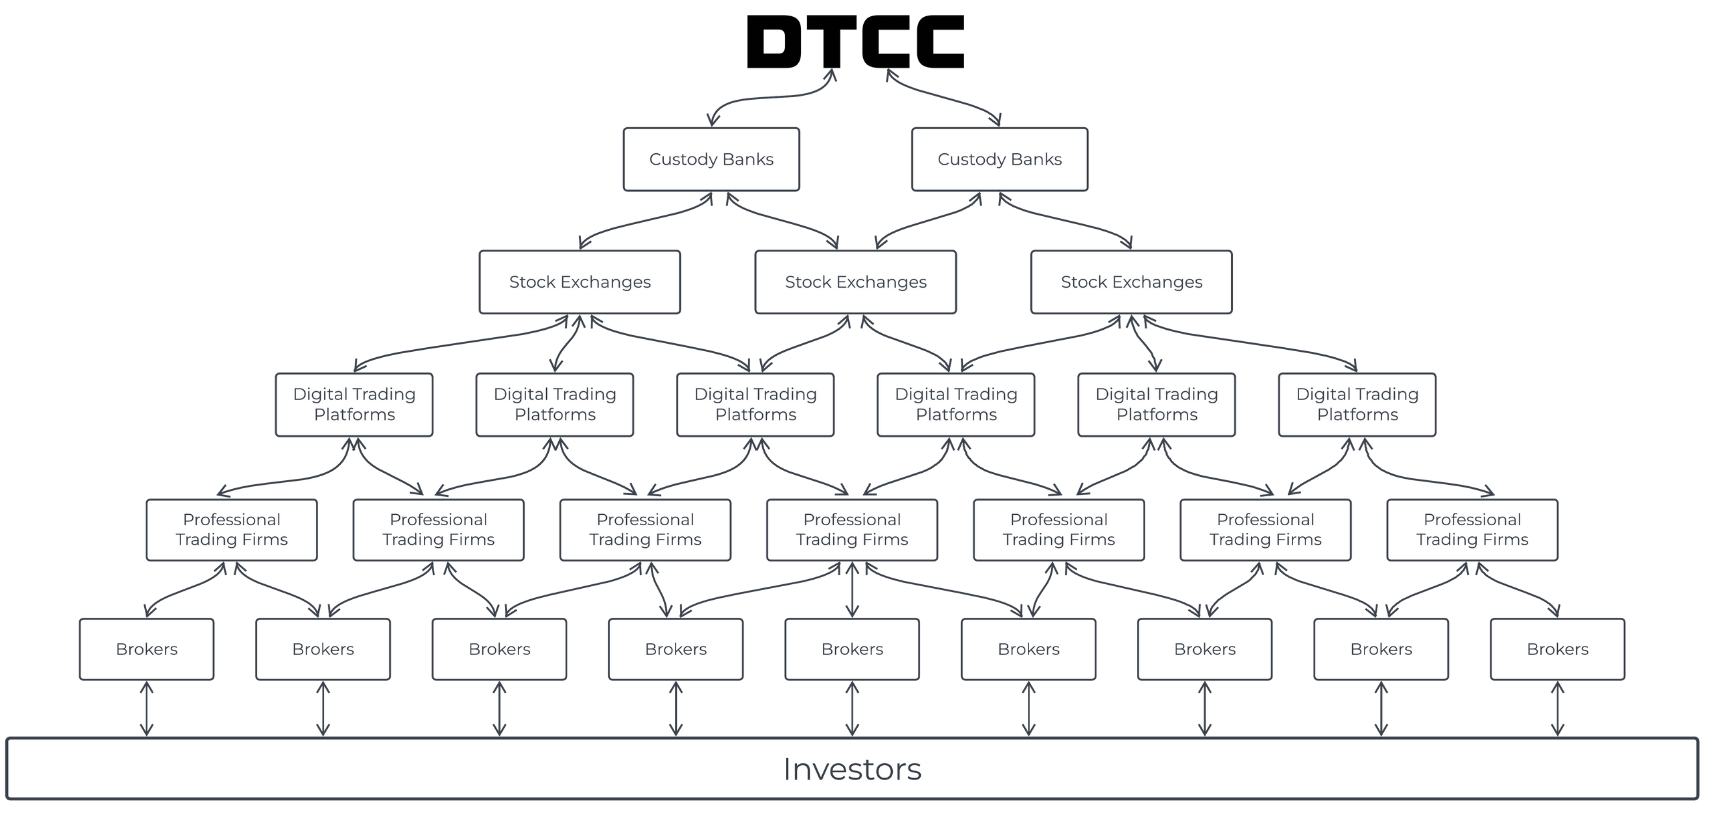
\includegraphics[width=455pt]{imgs/DTCC-pyramid.png}
    }
    \caption{Expanded View of Appendix \ref{appendix-intro}}
\end{figure}



\section{Ownership reconciliation shouldn't be this complex}\label{appendix-complex}

\begin{figure}[H]
    \centering
    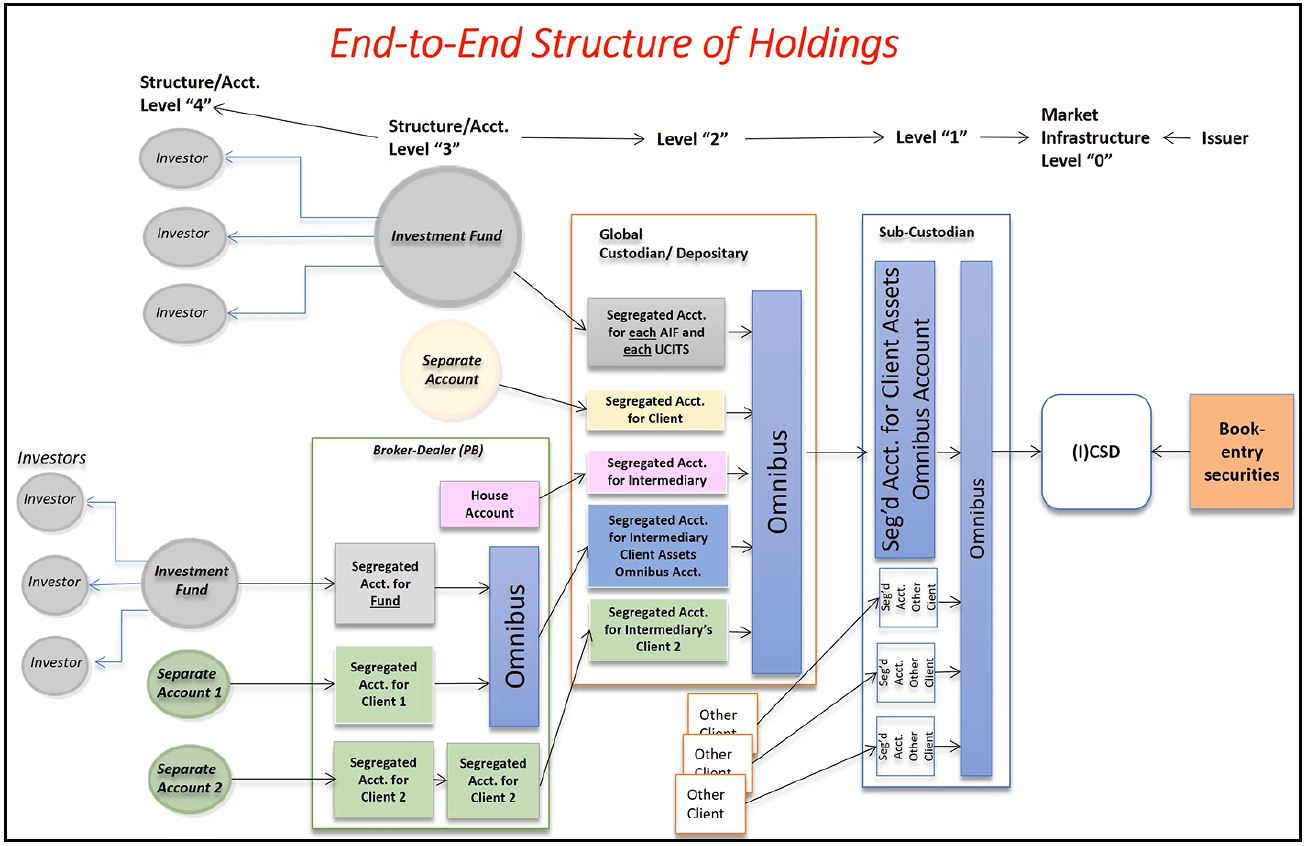
\includegraphics[width=475pt]{imgs/street-name.jpg}
    \caption{Expanded View of Appendix \ref{appendix-expanded}\cite{Infrastructure_2021}}
\end{figure}

\end{document}
